\chapter{СИСТЕМИЙН ШИНЖИЛГЭЭ БА ЗОХИОМЖ}

Энэ бүлэгт өмнөх бүлгүүдэд тодорхойлсон онолын хүрээ, судлагдсан байдлын дүгнэлтэд тулгуурлан зан үйлд суурилсан дадал төлөвшүүлэх системийн шинжилгээ, зохиомжийг боловсруулна. Тодруулбал, системийн зорилтот хэрэглэгчийн бүлэг, хамрах хүрээ, хэрэглэгчийн үүрэг, функциональ болон функциональ бус шаардлага, оролцогчид ба хэрэглээний тохиолдол, архитектурын зохион байгуулалт, өгөгдлийн загвар, үндсэн ажиллагааны логик, мөн туршилтын загварыг үнэлэх шалгуур, хэмжигдэх үзүүлэлтүүдийг системтэйгээр тодорхойлно. Энэ үе шатны үндсэн зорилго нь зан үйлийн онолын ойлголтуудыг програм хангамжийн системийн хэрэгжихүйц шийдэл болгон буулгаж, дараагийн хэрэгжүүлэлт, туршилт, үнэлгээний ажлын суурийг бүрдүүлэхэд оршино.

\section{Зорилтот хэрэглэгчийн бүлэг, хэрэглэгчийн үүрэг ба системийн хамрах хүрээ}

\subsection{Зорилтот хэрэглэгчийн бүлэг}

Туршилтын загварыг бүх насны, бүх төрлийн хэрэглэгчдэд нэгэн зэрэг зориулсан ерөнхий систем байхыг зорьсонгүй. Харин дадал төлөвшүүлэх хэрэгцээ өндөр, дижитал орчинд идэвхтэй, өдөр тутмын хуваарь, ачаалал, зорилгын өөрчлөлт ихтэй хэрэглэгчдийг зорилтот бүлэг болгон сонгов. Системийн үндсэн зорилтот хэрэглэгчийг ахлах ангийн сурагч, их, дээд сургуулийн оюутан, мөн ажлын гараагаа эхэлж буй залуу хэрэглэгчид гэж тодорхойлж байна. Насны хувьд эдгээр хэрэглэгчид нь ерөнхийдөө 16--30 насны хүрээнд хамаарна.

Зорилтот бүлгийг сонгосон нь хэд хэдэн үндэслэлтэй. Нэгдүгээрт, энэ үе шатны хэрэглэгчид суралцах дадал, цагийн менежмент, хувийн зохион байгуулалт, эрүүл амьдралын энгийн хэвшил зэрэг өдөр тутмын зан үйлийг тогтмолжуулах хэрэгцээ өндөртэй байдаг. Хоёрдугаарт, тэд дижитал хэрэглээний орчинд идэвхтэй тул сануулга, ахицыг хянах, санал сэтгэгдэл, урамшуулал зэрэг системийн механизмыг өдөр тутмын хэрэглээндээ шингээх боломж харьцангуй өндөр байна. Гуравдугаарт, амьдралын энэ үе шатанд шинэ орчин, шинэ үүрэг хариуцлага, цагийн ачааллын өөрчлөлт их байдаг тул зан үйлийг тогтворжуулах дэмжлэг бүхий систем практик ач холбогдолтой.

Системээр дэмжих дадлыг дараах үндсэн бүлгүүдэд авч үзэв.

\begin{table}[H]
\centering
\small
\setlength{\tabcolsep}{4pt}
\begin{tabular}{|L{3.5cm}|L{6.0cm}|L{4.0cm}|}
\hline
\textbf{Дадлын бүлэг} & \textbf{Тайлбар} & \textbf{Жишээ} \\
\hline
Суралцах дадал & Суралцах үйл ажиллагааг тогтмолжуулах дадал & Хичээл давтах, даалгавар хийх, ном унших \\
\hline
Хувийн зохион байгуулалтын дадал & Цаг, ажил, өдөр тутмын төлөвлөлттэй холбоотой дадал & Өдөр төлөвлөх, хийх ажлын жагсаалт гаргах \\
\hline
Эрүүл амьдралын хэвшлийн дадал & Бие, сэтгэл, эрүүл мэндтэй холбоотой энгийн дадал & Ус уух, дасгал хийх, цагтаа унтах \\
\hline
Өдөр тутмын тогтмол хэвшлийн дадал & Өдөр бүр давтагдах энгийн үйл ажиллагааны дадал & Өглөөний бэлтгэл, өрөө цэгцлэх, тогтмол цагт ажил эхлүүлэх \\
\hline
\end{tabular}
\caption{Системээр дэмжих дадлын үндсэн бүлгүүд}
\end{table}

Ийм ангилал нь системийн хамрах хүрээг тодорхой болгохоос гадна шаардлага, өгөгдлийн загвар, сануулгын логик, санал сэтгэгдлийн бүтэц зэрэг дараагийн шийдлүүдийг бодит хэрэглээтэй уялдуулах боломжийг бүрдүүлнэ.

\subsection{Хэрэглэгчийн үүрэг}

Системийн хүрээнд дараах үндсэн хэрэглэгчийн үүргийг авч үзэв.

\begin{table}[H]
\centering
\small
\setlength{\tabcolsep}{4pt}
\begin{tabular}{|L{3.0cm}|L{4.3cm}|L{6.2cm}|}
\hline
\textbf{Хэрэглэгчийн төрөл} & \textbf{Тодорхойлолт} & \textbf{Гол үйлдлүүд} \\
\hline
Үндсэн хэрэглэгч & Өөрийн дадлыг үүсгэж, тохируулж, өдөр тутмын гүйцэтгэлээ бүртгэн, ахицаа хянах хэрэглэгч & Дадал үүсгэх, засах, архивлах, өдөөгч дохио тохируулах, сануулга хүлээн авах, гүйцэтгэл бүртгэх, санал сэтгэгдэл оруулах, ахиц харах, урамшуулал болон ахицын мэдээллээ хуваалцах \\
\hline
\end{tabular}
\caption{Системийн үндсэн хэрэглэгчийн үүрэг}
\end{table}

Туршилтын загварын үндсэн хэрэглэгч нь үндсэн хэрэглэгч байна. Харин судалгааны хэрэгцээнд зориулсан нэмэлт удирдлагын боломжуудыг тусдаа, хязгаарлагдмал түвшинд авч үзнэ.

\subsection{Системийн хамрах хүрээ}

Системийн хамрах хүрээг тодорхойлох нь судалгааны ажлын хүрээнд ямар боломжуудыг хэрэгжүүлэх, мөн ямар боломжуудыг зориуд хамруулахгүй байхыг ялган тогтоох зорилготой. Энэ судалгаанд хамрах хүрээг зорилтот хэрэглэгчийн бодит хэрэглээ, туршилтын загварын түвшний хэрэгжих боломж, зан үйлийн дэмжлэгийн онолын шаардлагатай уялдуулан тодорхойлов.

\subsubsection*{Хамрах хүрээнд багтах зүйлс}

\begin{itemize}
    \item Хэрэглэгчийн бүртгэл, нэвтрэлт
    \item Дадал үүсгэх, засах, архивлах
    \item Дадлын идэвхтэй өдрүүд, эхлэх хугацаа, хэрэгжих хугацааны хүрээг тохируулах
    \item Дадал бүрт хэмжилтийн нэгж, доод зорилт, үндсэн зорилт тохируулах
    \item Дадал бүрт хувийн шалтгааны мэдээлэл хадгалах
    \item Цагийн хүрээ, ерөнхий байршил, өмнөх үйлдэл зэрэг өдөөгч нөхцөлийг тохируулах
    \item Дадлын үйлдэл, өдөөгч нөхцөл, шалтгаанд тулгуурласан өгүүлбэрэн урьдчилсан харагдац үзүүлэх
    \item Нөхцөл байдалд нийцсэн сануулга үүсгэх, илгээх, тайлбарлах
    \item Сануулгад өгсөн хэрэглэгчийн үйлдлийг бүртгэх
    \item Гүйцэтгэлийн бодит утга, бүртгэсэн хугацаа, эх үүсвэрийн ангиллыг хадгалах
    \item Бодит гүйцэтгэлийн утгыг доод зорилт болон үндсэн зорилттой харьцуулан үнэлэх
    \item Дадлыг жижиг алхмуудад хуваах
    \item Гүйцэтгэлийн дараах хэцүү байдлын үнэлгээ, эргэцүүлсэн санал сэтгэгдэл авах
    \item SRBAI-д суурилсан автоматжилтын үнэлгээ авах
    \item Тасралтгүй гүйцэтгэлийн цуваа, урамшуулал, дадлын хүчний оноо, ахицын шинжилгээ тооцоолох
    \item Урамшуулал болон ахицын мэдээллийг хуваалцах
    \item Хэрэглээний болон зан үйлийн шинжилгээний өгөгдөл бүртгэх
\end{itemize}

\subsubsection*{Хамрах хүрээнээс хасах зүйлс}

Судалгааны ажлын цар хүрээ, туршилтын загварын хэрэгжих боломж, дэвшилтэт вэб системийн техникийн хязгаарлалтыг харгалзан дараах боломжуудыг энэхүү ажлын хамрах хүрээнээс зориуд хасав.

\begin{itemize}
    \item зүүх төхөөрөмж, ухаалаг цагтай нэгтгэх боломж;
    \item өндөр нарийвчлалтай байршлын байнгын хяналт;
    \item төхөөрөмжийн доод түвшний мэдрэгчийн өгөгдөлд тулгуурласан зан үйлийн автоматаар таамаглах логик;
    \item машин сургалтад суурилсан бүрэн хувьсан өөрчлөгдөх сануулгын хөдөлгүүр;
    \item олон хэрэглэгчтэй нийгмийн харилцан дэмжлэг, өрсөлдөөнт орчин;
    \item зөвлөх, багш, сэтгэл зүйч зэрэг гуравдагч этгээдийн удирдлагын самбар;
    \item үйлдлийн системийн түвшний виджет, түгжээтэй дэлгэцийн тусгай удирдлага.
\end{itemize}

\section{Системийн шаардлагын шинжилгээ}

Энэ хэсэгт хэрэглэгчийн хэрэгцээ, онолын хүрээ, зан үйлийн дэмжлэгийн логик, техникийн боломж, хязгаарлалтыг нэгтгэн системийн шаардлага болгон тодорхойлно. Тодруулбал, дадал төлөвшлийн мөчлөг, Фоггийн зан үйлийн загвар, итгүүлэн нөлөөлөх технологийн зарчмууд, мөн дадлын хүчийг автоматжилтаар хэмжих хандлагыг програм хангамжийн системийн шаардлагад буулгасан болно.

\subsection{Функциональ шаардлага}

Функциональ шаардлага нь систем заавал ямар үйлдэл, үйлчилгээ, боломжуудыг агуулсан байхыг тодорхойлно. Энэ бүлэгт шаардлагыг ерөнхийлөн дараах логик багцуудаар нэгтгэв.

\begin{itemize}
    \item \textbf{Бүртгэл ба өгөгдлийн тусгаарлалт:} хэрэглэгч бүртгүүлэх, нэвтрэх, зөвхөн өөрийн өгөгдөлд хандах.
    \item \textbf{Дадлын удирдлага:} дадал үүсгэх, засах, архивлах, хуваарь болон хэмжилтийн тохиргоо хийх.
    \item \textbf{Өдөөгч нөхцөл ба сануулга:} нөхцөлд суурилсан сануулга үүсгэх, тайлбарлах, хэрэглэгчийн хариу үйлдлийг бүртгэх.
    \item \textbf{Гүйцэтгэл ба ахиц:} бодит гүйцэтгэл бүртгэх, зорилттой харьцуулан үнэлэх, цуваа болон ахиц тооцоолох.
    \item \textbf{Дасан зохицох дэмжлэг:} хэцүү байдлын үнэлгээ, эргэцүүлэл, хялбаршуулах санал, сануулгын бодлого шинэчлэх.
    \item \textbf{Автоматжилт ба дадлын хүч:} SRBAI үнэлгээ авах, дадлын хүчний оноо тооцоолох, бэхжилтийн түвшин хянах.
    \item \textbf{Шинжилгээ ба хуваалцах:} судалгааны үзүүлэлтэд шаардлагатай лог бүртгэх, ахиц ба урамшууллыг хуваалцах.
\end{itemize}

Функциональ шаардлагын бүрэн жагсаалт, кодчилол, баталгаажуулах шалгуурыг Хавсралт A-д дэлгэрэнгүй хүснэгтээр өгсөн (Хүснэгт~\ref{app:functional-1}, Хүснэгт~\ref{app:functional-2}).

\subsection{Сануулгын цаг сонголттой холбоотой шаардлагын тайлбар}

Уг системийн онцлог нь сануулгыг зөвхөн тогтмол цагт илгээх энгийн дүрмээр бус, харин хуваарь, өдөөгч нөхцөл, өмнөх хариу үйлдэл, тухайн өдрийн гүйцэтгэлийн төлөв, мөн сануулгын бодлогын одоогийн түвшнийг хамтатган авч үзэхэд оршино. Иймээс сануулга илгээх шийдвэр нь дараах үндсэн шалгууруудад тулгуурлана. Үүнд тухайн өдөр дадал идэвхтэй эсэх, өдрийн тохирох цагийн хүрээнд байгаа эсэх, уг дадал аль хэдийн бүртгэгдсэн эсэх, ижил нөхцөлд өмнө нь ямар хариу өгч байсан эсэх, мөн сануулгыг аажмаар бууруулах бодлогын дагуу тухайн мөчид сануулах шаардлагатай эсэх зэрэг орно.

\subsection{Функциональ бус шаардлага}

Функциональ бус шаардлага нь системийн чанар, найдвартай байдал, ашиглахад хялбар байдал, нууцлал зэрэг үзүүлэлтийг тодорхойлно.

\begin{longtable}{|L{1.1cm}|L{2.8cm}|L{5.5cm}|L{3.5cm}|}
\hline
\textbf{Код} & \textbf{Ангилал} & \textbf{Функциональ бус шаардлага} & \textbf{Хэмжигдэх шалгуур} \\
\hline
\endhead
ФБШ-01 & Ашиглахад хялбар байдал & Үндсэн хэрэглээний урсгалууд ойлгомжтой, цөөн алхамтай байх ёстой. & Сануулгаас гүйцэтгэл бүртгэх үйлдэл 1 товшилтоор, үндсэн дэлгэцээс 2-оос ихгүй алхмаар хийгдэх \\
\hline
ФБШ-02 & Гүйцэтгэл & Гол дэлгэцүүд болон чухал үйлдлүүд богино хугацаанд хариу өгөх ёстой. & Гол дэлгэц ачаалах хугацаа 2 секундээс ихгүй, гүйцэтгэл хадгалах хугацаа 1 секундээс ихгүй \\
\hline
ФБШ-03 & Найдвартай байдал & Гүйцэтгэлийн бүртгэл, сануулгын үйлдэл, урамшууллын мэдээлэл, автоматжилтын үнэлгээ алдагдалгүй хадгалагдах ёстой. & Туршилтын өгөгдлийн бүрэн бүтэн байдал 100 хувь байх \\
\hline
ФБШ-04 & Аюулгүй байдал & Хэрэглэгчийн өгөгдлийг зөвшөөрөлгүй хандалтаас хамгаалах ёстой. & Нууц үгийг хэш хэлбэрээр хадгалах, баталгаажсан хандалт шаардах \\
\hline
ФБШ-05 & Нууцлал & Систем зөвхөн шаардлагатай хамгийн бага нөхцөл байдлын мэдээллийг ашиглах ёстой. & Байршлын өгөгдөл ерөнхий ангиллын түвшинд хадгалагдах \\
\hline
ФБШ-06 & Тохирох чадвар & Систем түгээмэл орчин үеийн хөтөч болон хөдөлгөөнт орчинд ажиллах ёстой. & Chrome, Edge, Safari дээр үндсэн урсгалууд алдаагүй ажиллах \\
\hline
ФБШ-07 & Засварлах ба өргөтгөх чадвар & Системийн бүтэц нь модульчилсан, өргөтгөх, засварлахад хялбар байх ёстой. & Интерфэйс, хэрэглээний логик, домайн логик, өгөгдлийн түвшин тусгаарлагдсан байх \\
\hline
ФБШ-08 & Ачаалал даах чадвар & Туршилтын түвшинд өгөгдлийн хэмжээ өсөхөд үндсэн ажиллагаа тогтвортой байх ёстой. & Олон дадал, олон бүртгэлтэй өгөгдөл дээр ажиллагаа хэвийн үргэлжлэх \\
\hline
ФБШ-09 & Ажиглагдах чадвар & Судалгааны үзүүлэлтүүдийг тооцоход хангалттай аналитик өгөгдөл бүртгэгдэх ёстой. & Хэрэглээний болон зан үйлийн үзүүлэлтүүдийг тооцох боломжтой байх \\
\hline
ФБШ-10 & Алдаа зохицуулалт & Алдаа гарсан үед систем ойлгомжтой мэдээлэл өгч, өгөгдлийг буруу төлөвт оруулахгүй байх ёстой. & Алдааны мэдээлэл, дахин оролдох логик ажиллах \\
\hline
\end{longtable}

Эдгээр чанарын шаардлага нь зөвхөн техникийн найдвартай ажиллагаанд бус, мөн зан үйлийн дэмжлэгийг саад багатай хэрэгжүүлэхэд чиглэж байна. Ялангуяа ашиглахад хялбар байдал, төвөгшил багатай харилцан үйлчлэл, нууцлалыг хамгаалсан нөхцөл байдлын загварчлал нь уг судалгааны суурь концепцтэй шууд уялдана.

\section{Системийн оролцогчид ба хэрэглээний тохиолдол}

Уг системийн хэрэглээний тохиолдлын үндсэн оролцогч нь хэрэглэгч болно. Харин сануулга үүсгэх, урамшуулал идэвхжүүлэх, шинжилгээний үзүүлэлт тооцоолох, дадлын хүчний оноо үнэлэх, сануулгын бодлого шинэчлэх зэрэг нь системийн дотоод автомат логикоор хэрэгжих тул хэрэглээний тохиолдлын диаграммд тусдаа гадаад оролцогч болгон дүрслэхгүй.

\subsection{Үндсэн хэрэглээний тохиолдлууд}

\begin{table}[H]
\centering
\small
\setlength{\tabcolsep}{4pt}
\begin{tabular}{|L{5.5cm}|L{7.5cm}|}
\hline
\textbf{Хэрэглээний тохиолдол} & \textbf{Тайлбар} \\
\hline
Бүртгүүлэх, нэвтрэх & Хэрэглэгч системд бүртгүүлж, хувийн орчин руу нэвтрэх \\
\hline
Дадал үүсгэх & Дадлын нэр, зорилго, хуваарь, хэмжилт, өдөөгч нөхцөл, шалтгааны мэдээллийг тохируулах \\
\hline
Өдөөгч нөхцөл тохируулах & Цаг, байршил зэрэг нөхцөлийг тохируулах \\
\hline
Сануулга хүлээн авах & Систем нөхцөл байдалд тулгуурлан сануулга илгээх \\
\hline
Сануулгын үйлдэл сонгох & ``Хийлээ'', ``дараа сануул'' зэрэг үйлдэл сонгох \\
\hline
Гүйцэтгэл бүртгэх & Дадлын гүйцэтгэлийг хэмжээгээр бүртгэх \\
\hline
Автоматжилтын үнэлгээ өгөх & SRBAI-д суурилсан асуулгад хариулах \\
\hline
Ахиц харах & Гүйцэтгэлийн түүх, цуваа, оноо, шинжилгээний мэдээлэл харах \\
\hline
Санал сэтгэгдэл өгөх & Хэцүү байдал, анхаарал, эрч хүч, сэтгэл санаа, ашиг тусын мэдээлэл оруулах \\
\hline
Ахиц, урамшууллаа хуваалцах & Ахицын карт, урамшуулал, амжилтын мэдээллийг бусадтай хуваалцах \\
\hline
\end{tabular}
\caption{Системийн үндсэн хэрэглээний тохиолдлууд}
\end{table}

\begin{figure}[H]
    \centering
    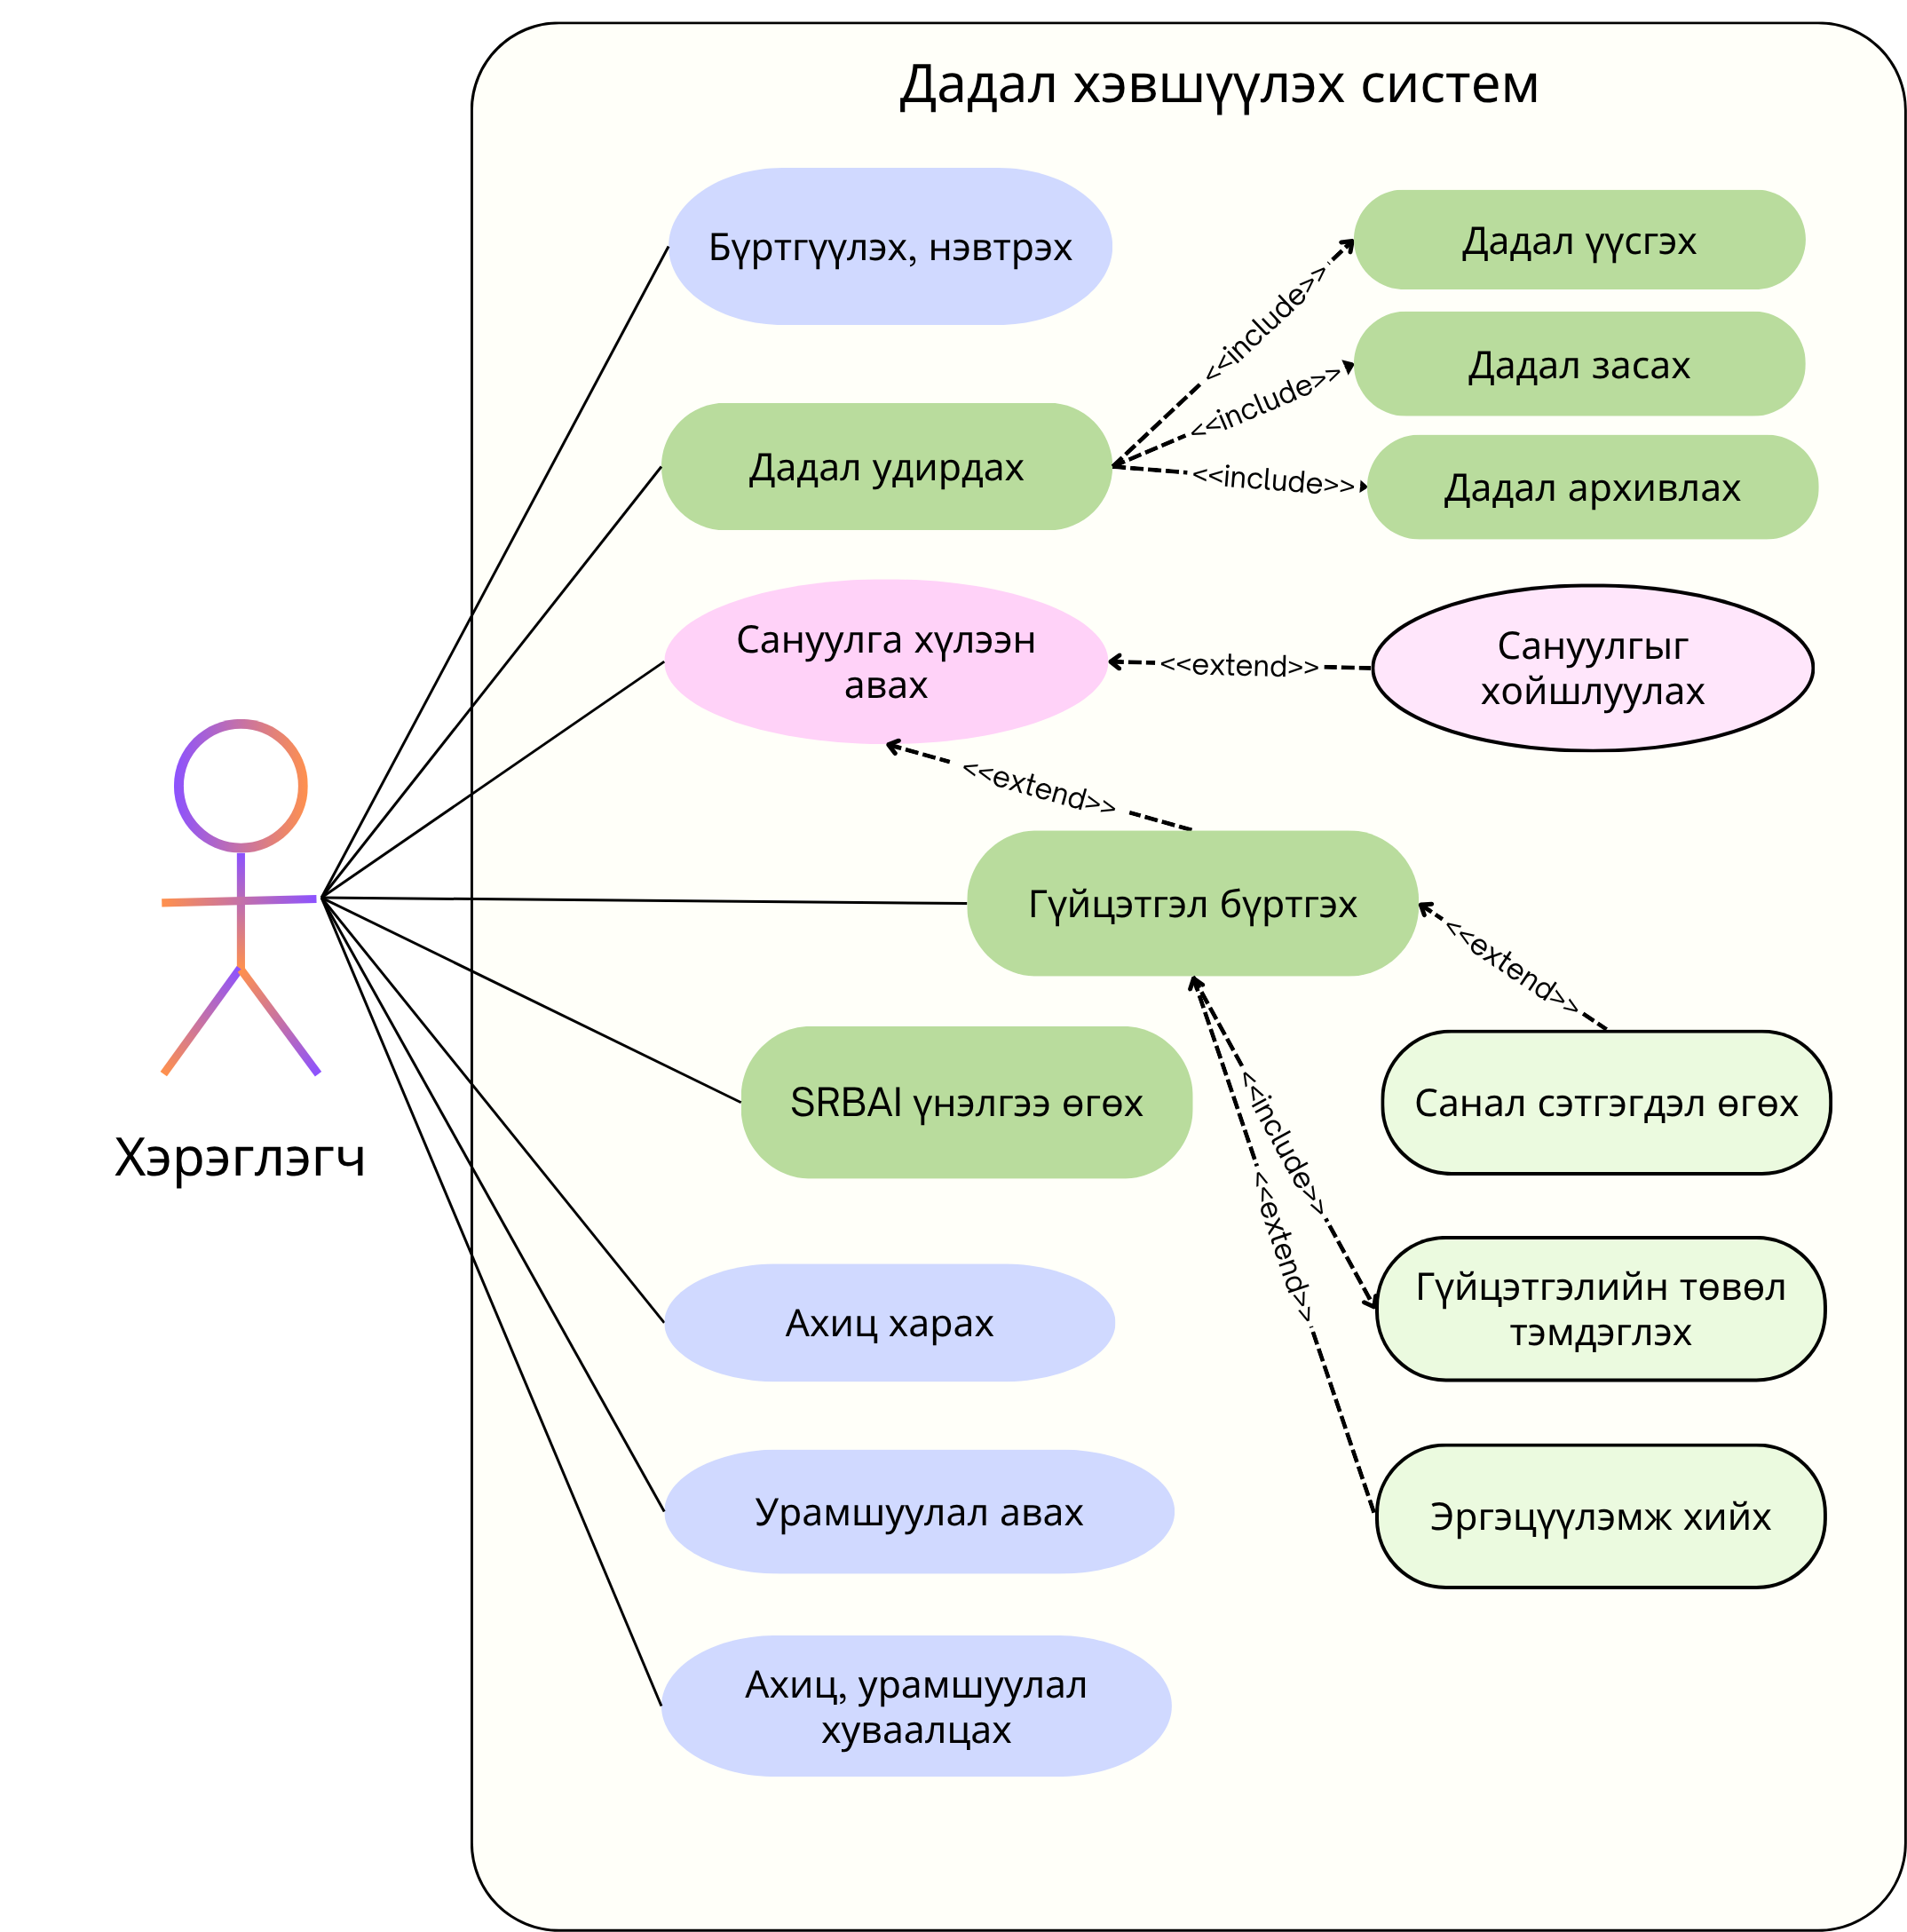
\includegraphics[width=0.72\textwidth]{images/GeneralUseCaseDiagram.png}
    \caption{Системийн ерөнхий хэрэглээний тохиолдлын диаграмм}
\end{figure}

\section{Системийн архитектурын зохиомж}

\subsection{Ерөнхий архитектур}

Туршилтын загварын архитектурыг хэрэгжүүлэх боломж, системийн төвөгшлийн түвшин, судалгааны ажлын цар хүрээг харгалзан клиент--сервер хэв маягтай, сервер талдаа модульчилсан нэг бүхэл архитектуртай, дотоод зохион байгуулалтын түвшинд цэвэр архитектурын зарчмыг баримталсан байдлаар зохиомжлов. Өөрөөр хэлбэл, систем нь байршуулалтын түвшинд нэг серверийн бүрэлдэхүүнтэй ажиллах боловч доторх логик нь үүргээрээ тусгаарлагдсан модулиудад хуваагдана.

Системийн хэрэглэгчийн тал нь React дээр хэрэгжсэн дэвшилтэт вэб програм (PWA) байна. Энэ нь веб болон хөдөлгөөнт орчинд ижил суурьтай хэрэглээний туршлага өгөхөөс гадна үйлчилгээний ажиллагчийн тусламжтайгаар вэб мэдэгдэл, хязгаарлагдмал оффлайн дэмжлэгийг хэрэгжүүлэх боломж бүрдүүлнэ. Сервер тал нь NestJS дээр хэрэгжих бөгөөд бүртгэл ба хандалт, дадлын удирдлага, өдөөгч нөхцөл ба хуваарь, сануулгын шийдвэрийн логик, гүйцэтгэл ба ахиц, санал сэтгэгдэл ба урамшуулал, дадал бэхжилтийн үнэлгээ, шинжилгээний модуль зэрэг үндсэн бүрэлдэхүүнүүдийг агуулна. Өгөгдлийн үндсэн сан нь PostgreSQL байх бөгөөд хуваарьт ажлын үйлчилгээ сануулгын дүрэмт логикийг хугацааны дагуу ажиллуулна.

Системийн ерөнхий архитектурын давхаргат зохион байгуулалтыг дараах зурагт үзүүлэв.

\begin{figure}[H]
    \centering
    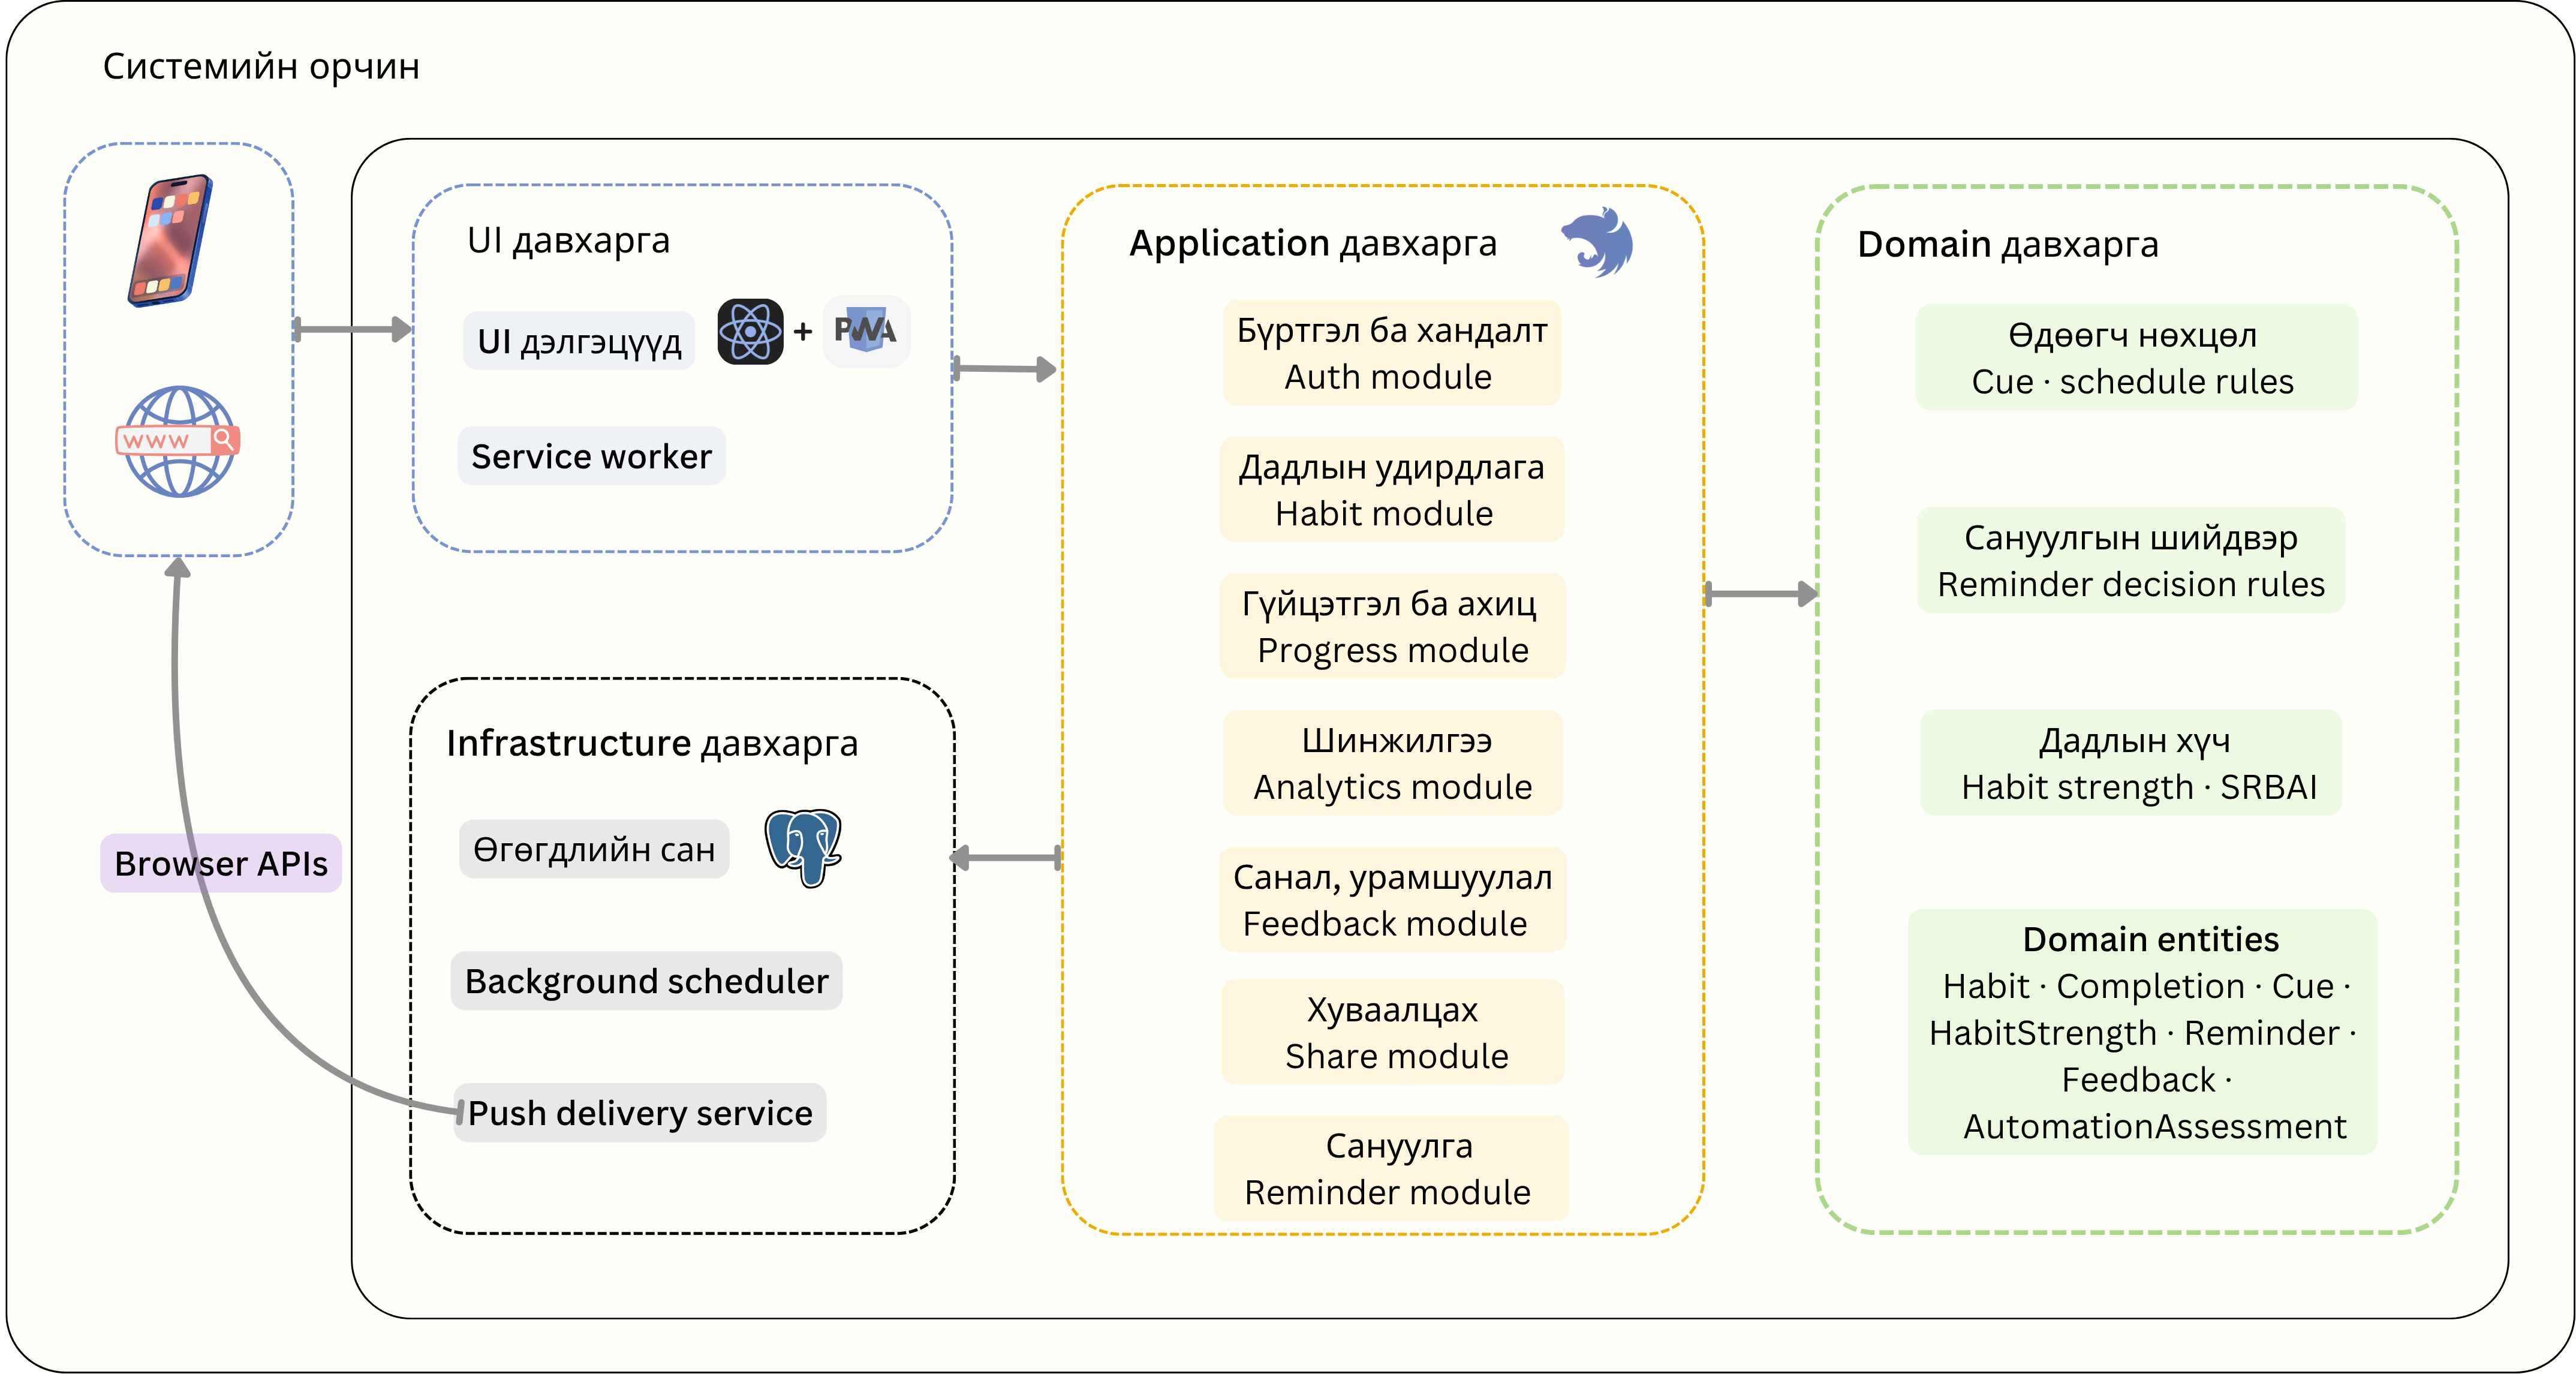
\includegraphics[width=0.96\textwidth]{images/CleanArchitectureDiagram.png}
    \caption{Системийн ерөнхий архитектур}
\end{figure}

\subsection{Архитектурын давхаргууд}

\begin{table}[htbp]
\centering
\small
\setlength{\tabcolsep}{4pt}
\begin{tabular}{|L{4.1cm}|L{8.9cm}|}
\hline
\textbf{Давхарга} & \textbf{Үндсэн үүрэг} \\
\hline
Хэрэглэгчийн интерфэйсийн түвшин & Дэлгэц, урсгал, компонент, хэрэглэгчийн шууд харилцан үйлчлэлийг хариуцах \\
\hline
Хэрэглээний логикийн түвшин & Модулиудын хэрэглээний урсгал, API, үйлчилгээний уялдаа холбоог хариуцах \\
\hline
Домайн логикийн түвшин & Системийн үндсэн дүрэм, хязгаарлалт, тооцооллын логикийг агуулна \\
\hline
Өгөгдөл ба дэд бүтцийн түвшин & Өгөгдөл хадгалах, гадаад үйлчилгээтэй холбогдох, мэдэгдэл хүргэх дэд бүтцийг хариуцна \\
\hline
\end{tabular}
\caption{Архитектурын давхаргууд}
\end{table}

\subsection{Хэрэглээний логикийн үндсэн модулиуд}

\begin{table}[htbp]
\centering
\small
\setlength{\tabcolsep}{4pt}
\begin{tabular}{|L{4.2cm}|L{8.8cm}|}
\hline
\textbf{Модуль} & \textbf{Үндсэн үүрэг} \\
\hline
Бүртгэл ба хандалтын модуль & Хэрэглэгчийн бүртгэл, нэвтрэлт, эрхийн шалгалтыг хариуцах \\
\hline
Дадлын удирдлагын модуль & Дадал үүсгэх, засах, архивлах, үндсэн шинжүүдийг удирдах \\
\hline
Өдөөгч нөхцөл ба хуваарийн модуль & Өдрийн цаг, өдрийн төрөл, нөхцөл байдал, хуваарийн мэдээллийг удирдах \\
\hline
Сануулгын модуль & Сануулга илгээх шаардлагатай эсэхийг дүрэмт логикоор шийдвэрлэх \\
\hline
Мэдэгдэл хүргэх модуль & Сануулгын мэдээллийг мэдэгдлийн дэд бүтцээр дамжуулан хүргэх \\
\hline
Гүйцэтгэл ба ахицын модуль & Гүйцэтгэл бүртгэх, цуваа тооцох, ахицын мэдээлэл гаргах \\
\hline
Санал сэтгэгдэл ба урамшууллын модуль & Санал сэтгэгдэл, урамшуулал, эргэцүүллийн мэдээллийг хариуцах \\
\hline
Дадлын хүчний модуль & Автоматжилтын үнэлгээ боловсруулах, нийлмэл оноо тооцоолох, бэхжилтийн түвшин үнэлэх \\
\hline
Шинжилгээний модуль & Хэрэглээний болон зан үйлийн үзүүлэлтүүдийг тооцоолох \\
\hline
Хуваалцах дэмжлэгийн модуль & Ахиц, урамшууллыг гадна орчинд хуваалцах урсгалыг дэмжих \\
\hline
\end{tabular}
\caption{Хэрэглээний логикийн үндсэн модулиуд}
\end{table}

Эдгээр модулиудын дундаас сануулгын модуль болон дадлын хүчний модуль нь уг системийн зан үйлийн дэмжлэгийн гол цөм болно. Сануулгын модуль нь өдөөгч нөхцөл, гүйцэтгэлийн түүх, сануулгад өгсөн үйлдлийн түүх, сануулгыг аажмаар бууруулах бодлого зэрэг мэдээлэлд тулгуурлан тухайн мөчид сануулга илгээх эсэхийг шийдвэрлэнэ. Харин дадлын хүчний модуль нь автоматжилтын үнэлгээ, гүйцэтгэлийн тогтвортой байдал, өдөөгч нөхцлийн тогтвортой байдал зэрэг мэдээлэлд тулгуурлан тухайн дадлын бэхжилтийн түвшнийг үнэлнэ. Модулиудын харилцан уялдаа нь дээр дурдсан ерөнхий архитектур болон хүснэгтэн тодорхойлолтуудад нэгтгэн тусгагдсан.

\subsection{Мэдэгдэл хүргэх механизм}

Архитектурын нэг чухал онцлог нь мэдэгдэл хүргэх логикийг хэрэглэгчийн интерфэйсээс тусад нь зохион байгуулсан явдал юм. Сануулгын модуль нь тухайн мөчид сануулга илгээх шаардлагатай гэж үзсэн тохиолдолд мэдэгдэл хүргэх бүрэлдэхүүнд мэдээлэл дамжуулна. Улмаар уг бүрэлдэхүүн нь вэб мэдэгдлийн дэд бүтцээр дамжуулан хэрэглэгчийн төхөөрөмж рүү сануулга илгээнэ.

Хэрэглэгчийн интерфэйс тухайн үед нээлттэй биш байсан ч үйлчилгээний ажиллагч мэдэгдлийг хүлээн авч, хөтөч эсвэл үйлдлийн системийн мэдэгдлийн орчинд харуулах боломжтой. Хэрэглэгч мэдэгдэл дээрээс шууд үйлдэл сонгосон тохиолдолд тухайн мэдээлэл сервер тал руу буцаж дамжин, сануулгын үйлдэл болон дараах гүйцэтгэлийн урсгалтай холбогдоно.

\section{Өгөгдлийн загварын зохиомж}

Системийн өгөгдлийн загвар нь дадал төлөвшлийн үйл явцыг зөвхөн ``хийсэн'' эсэхээр бус, харин ``ямар нөхцөлд'', ``ямар өдөөлтөөр'', ``ямар хариу үйлдэлтэйгээр'', ``ямар санал сэтгэгдэлтэйгээр'', мөн ``хэр зэрэг автоматжиж буй''-г системтэй хадгалах зорилготой. Үүний тулд дараах үндсэн өгөгдлийн нэгжүүдийг тодорхойлов.

\begin{table}[htbp]
\centering
\small
\setlength{\tabcolsep}{4pt}
\begin{tabular}{|L{4.6cm}|L{8.4cm}|}
\hline
\textbf{Өгөгдлийн нэгж} & \textbf{Тайлбар} \\
\hline
Хэрэглэгч & Системийн хэрэглэгчийн үндсэн мэдээлэл \\
\hline
Дадал & Хэрэглэгчийн хэрэгжүүлэх зан үйлийн үндсэн мэдээлэл, хуваарь, хэмжилтийн тохиргоог хадгална. \\
\hline
Шалтгаан & Тухайн дадлыг яагаад хэрэгжүүлэх гэж буй хувийн шалтгааны мэдээллийг хадгална. \\
\hline
Өдөөгч нөхцөл & Цагийн хүрээ, ерөнхий байршил, өмнөх үйлдэл зэрэг сануулгын шийдвэрт ашиглагдах нөхцөлийг хадгална. \\
\hline
Хуваарийн өдөр & Дадал аль өдрүүдэд идэвхтэй байхыг илэрхийлэх өгөгдөл \\
\hline
Жижиг алхам & Дадлыг хэрэгжүүлэхэд зориулсан жижиг алхмууд \\
\hline
Сануулга & Илгээсэн сануулгын бүртгэл \\
\hline
Сануулгын үйлдэл & Сануулгад өгсөн хэрэглэгчийн үйлдэл \\
\hline
\end{tabular}
\caption{Системийн үндсэн өгөгдлийн нэгжүүд (I)}
\end{table}

\begin{table}[htbp]
\centering
\small
\setlength{\tabcolsep}{4pt}
\begin{tabular}{|L{4.6cm}|L{8.4cm}|}
\hline
\textbf{Өгөгдлийн нэгж} & \textbf{Тайлбар} \\
\hline
Гүйцэтгэлийн бүртгэл & Бодит гүйцэтгэлийн утга, бүртгэсэн хугацаа, гүйцэтгэлийн эх үүсвэр, доод зорилт хангасан эсэх, үндсэн зорилт хүрсэн эсэхийг хадгална. \\
\hline
Хэцүү байдлын үнэлгээ & Гүйцэтгэлийн дараах төвөгшлийн үнэлгээг хадгална. \\
\hline
Эргэцүүлсэн санал сэтгэгдэл & Гүйцэтгэлийн дараах ашиг тусын талаарх товч эргэцүүллийг хадгална. \\
\hline
Автоматжилтын үнэлгээ & SRBAI-д суурилсан асуулгын хариулт, тооцоолсон оноо \\
\hline
Урамшууллын үйл явдал & Оноо, тэмдэг, баяр хүргэлт зэрэг урамшууллын бүртгэл \\
\hline
Дадлын хүч & Дадлын тогтворжилтын нийлмэл оноо, түвшний хадгалалт \\
\hline
Интерфэйсийн үйл явдлын бүртгэл & Микро түвшний хэрэглээний үйлдлийн бүртгэл \\
\hline
Хэрэглэгчийн үйл ажиллагааны бүртгэл & Апп нээх, ажиллагааны үе эхлүүлэх, ажиллагааны үе дуусгах зэрэг системийн ерөнхий хэрэглээний идэвхийг хадгална. \\
\hline
\end{tabular}
\caption{Системийн үндсэн өгөгдлийн нэгжүүд (II)}
\end{table}

Өгөгдлийн хамаарлын бүтэц дээр дадал нь төв нэгж болно. Нэг хэрэглэгч олон дадалтай байж болох бөгөөд дадал бүр нэг шалтгааны мэдээлэлтэй, олон өдөөгч нөхцөл, олон идэвхтэй өдөр, олон жижиг алхам, олон сануулга, олон гүйцэтгэлийн бүртгэлтэй холбогдоно. Гүйцэтгэлийн бүртгэл бүр нь хэцүү байдлын үнэлгээ, эргэцүүлсэн санал сэтгэгдэл, урамшууллын үйл явдалтай уялдах боломжтой. Мөн автоматжилтын үнэлгээ болон дадлын хүчний оноо нь хугацааны явцад олон удаа бүртгэгдэх тул тухайн дадлын өөрчлөлтийн чиг хандлалыг хугацааны дарааллаар шинжлэх боломж бүрдэнэ.

\section{Хэрэглэгчийн интерфэйс ба хэрэглээний туршлагын зохиомж}

Дадал үүсгэх дэлгэц нь хэрэглэгчээс олон салангид, төвөгтэй талбар бөглүүлэхийн оронд үндсэн гурван ойлголтыг төв болгон зохиомжилсон. Үүнд: юу хийх вэ, хэзээ эсвэл ямар нөхцөлд хийх вэ, яагаад хийх вэ гэсэн мэдээлэл орно. Систем нь эдгээр оролтод тулгуурлан хэрэглэгчид ойлгомжтой өгүүлбэрэн урьдчилсан харагдац үзүүлнэ. Жишээлбэл, ``Сэрснийхээ дараа би 5 минут бясалгал хийнэ. Шалтгаан: өдрийг тайван эхлүүлэхийн тулд.'' гэсэн хэлбэрийн урьдчилсан харагдац нь хэрэглэгчийн оруулсан мэдээллийг нэг мөр ойлгож, баталгаажуулахад дэмжлэг үзүүлнэ. Ийнхүү интерфэйс нь өгөгдлийг бүтцэт байдлаар хадгалж байгаа боловч хэрэглэгчид байгалийн хэллэгт ойр, ойлгомжтой хэлбэрээр харуулах зарчмыг баримтална.

\section{Системийн ажиллагааны үндсэн логик}

\providecommand{\systemdiagram}[2]{%
\begin{figure}[H]
    \centering
    \includegraphics[width=\textwidth,height=0.82\textheight,keepaspectratio]{#1}
    \caption{#2}
\end{figure}
}

Системийн ажиллагааны үндсэн логик нь дадал төлөвшлийн мөчлөгийн дараалалтай нийцсэн байдлаар зохион байгуулагдсан. Өөрөөр хэлбэл, систем нь хэрэглэгчийн зан үйлийг зөвхөн бүртгэх бус, харин эхлүүлэх, хэрэгжүүлэх, бататгах, аажмаар тогтворжуулах чиглэлээр дэмжинэ.

\subsection{Үндсэн урсгал}

Системийн ажиллагааны үндсэн урсгал дараах байдалтай байна. Нэгдүгээрт, хэрэглэгч шинэ дадал үүсгэж, түүнд хамаарах зорилго, өдөөгч нөхцөл, хуваарь, шаардлагатай бол жижиг алхмуудыг тохируулна. Хоёрдугаарт, систем эдгээр мэдээлэлд тулгуурлан сануулгын логикийг бэлтгэнэ. Гуравдугаарт, тохирох нөхцөл бүрдсэн үед сануулгын модуль сануулга илгээх эсэхийг шийдвэрлэж, шаардлагатай бол мэдэгдэл хүргэх модуль рүү дамжуулна. Дөрөвдүгээрт, хэрэглэгч сануулгад үйлдэл сонгож, эсвэл өөрийн санаачилгаар гүйцэтгэл бүртгэнэ. Тавдугаарт, гүйцэтгэлийн дараа урамшуулал, санал сэтгэгдэл, эргэцүүллийн урсгал идэвхжинэ. Зургаадугаарт, систем хуримтлагдсан өгөгдөлд тулгуурлан ахиц, цуваа, автоматжилтын түвшин, дадлын хүчний оноо, сануулгаас хараат бус байдлын үзүүлэлтийг тооцоолно. Долоодугаарт, дадал тогтворжихын хэрээр сануулгын давтамжийг аажмаар бууруулж, хэрэглэгчийн өөрийн санаачилгатай зан үйлийг дэмжинэ.

Системийн үндсэн ажиллагааны дарааллыг дээрх урсгалын тайлбарт үе шат бүрээр нь нэгтгэн үзүүлэв.

\noindent Үндсэн системийн урсгалын үйл ажиллагааны диаграмм.
Энэхүү үйл ажиллагааны диаграмм нь системийн ерөнхий урсгалыг хэрэглэгчийн дадал үүсгэхээс эхлэн сануулга, гүйцэтгэл бүртгэл, санал сэтгэгдэл, ахицын тооцоолол, сануулгын бодлогын шинэчлэлт хүртэлх дарааллаар үзүүлж байна.

\systemdiagram{images/ActivityDiagram1.png}{Дадал төлөвшүүлэх системийн үндсэн үйл ажиллагааны урсгал}

Дадал үүсгэх, тохируулах, хадгалах дарааллын нарийвчилсан харилцан үйлчлэлийн диаграммыг хавсралтад үзүүлэв.

\subsection{Дадал төлөвшлийн мөчлөг ба системийн хэрэгжилтийн уялдаа}

\begin{table}[htbp]
\centering
\small
\setlength{\tabcolsep}{4pt}
\begin{tabular}{|L{4.8cm}|L{8.2cm}|}
\hline
\textbf{Дадал төлөвшлийн мөчлөгийн үе шат} & \textbf{Системийн хэрэгжилт} \\
\hline
Өдөөгч дохио & Нөхцөл байдалд суурилсан сануулга, өдөөгч нөхцлийн тохиргоо, сануулгын тайлбар \\
\hline
Хүсэл тэмүүлэл & Хувийн шалтгаан, зорилгын утгыг эргэн сануулах мэдээлэл \\
\hline
Хариу үйлдэл & ``Хийсэн'', ``хэсэгчлэн хийсэн'' бүртгэл, нэг товшилтын урсгал, жижиг алхам, хялбаршуулах дэмжлэг \\
\hline
Урамшуулал & Оноо, баяр хүргэлт, тасралтгүй гүйцэтгэлийн цуваа, эргэцүүлсэн санал сэтгэгдэл \\
\hline
Бэхжилт ба автоматжилт & SRBAI үнэлгээ, дадлын хүчний оноо, сануулгын бодлогын өөрчлөлт \\
\hline
\end{tabular}
\caption{Дадал төлөвшлийн мөчлөг ба системийн хэрэгжилтийн уялдаа}
\end{table}

Энэхүү уялдаа нь онолын загвар системийн функц, өгөгдлийн бүтэц, харилцан үйлчлэлийн урсгалын түвшинд бодитоор тусгагдсан болохыг харуулна.

\subsection{Сануулгаас хараат бус байдлыг хянах логик}

Уг системийн ялгарах нэг онцлог нь гүйцэтгэлийн эх үүсвэрийг ангилан бүртгэх явдал юм. Өөрөөр хэлбэл, хэрэглэгчийн гүйцэтгэл сануулгын шууд нөлөөгөөр хийгдсэн үү, эсвэл хэрэглэгч өөрийн санаачилгаар хийсэн үү гэдгийг ялган хадгална. Үүний тулд гүйцэтгэлийн бүртгэл бүр дээр эх үүсвэрийн ангилал хадгална. Үүнд сануулгад тулгуурласан, өөрийн санаачилгатай, тодорхойгүй гэсэн ангиллууд орно.

Хэрэв хэрэглэгч сануулгад үйлдэл сонгосны дараа богино хугацаанд гүйцэтгэл бүртгэсэн бол тухайн үйлдлийг сануулгад тулгуурласан гэж ангилна. Харин хэрэглэгч сануулгагүй үед системийг өөрөө нээн гүйцэтгэл бүртгэсэн бол өөрийн санаачилгатай гэж ангилна. Энэ ангилал нь сануулгаас хэт хараат байдлыг үнэлэх, дадал аажмаар дотооджиж байгаа эсэхийг шинжлэх суурь өгөгдөл болно.

Сануулгыг нөхцөл байдалд тулгуурлан шийдвэрлэх дүрэмт логик нь өдрийн идэвхтэй хуваарь, цагийн хүрээ, өмнөх гүйцэтгэл, хүлээлгийн хугацаа болон сануулгын бодлогын нөхцөлийг хамтатган авч үздэг. Энэ урсгалын үйл ажиллагааны болон дарааллын дэлгэрэнгүй диаграммуудыг хавсралтад оруулав.

\begin{table}[htbp]
\centering
\small
\setlength{\tabcolsep}{4pt}
\begin{tabular}{|L{6.5cm}|L{6.5cm}|}
\hline
\textbf{Нөхцөл} & \textbf{Ангиллын шийдвэр} \\
\hline
Хэрэглэгч сануулгад үйлдэл сонгосны дараа богино хугацаанд гүйцэтгэл бүртгэсэн & Сануулгад тулгуурласан гүйцэтгэл \\
\hline
Хэрэглэгч сануулгагүйгээр системийг өөрөө нээж гүйцэтгэл бүртгэсэн & Өөрийн санаачилгатай гүйцэтгэл \\
\hline
Эх үүсвэрийг тодорхой ялгах боломжгүй & Тодорхойгүй эх үүсвэр \\
\hline
\end{tabular}
\caption{Гүйцэтгэлийн эх үүсвэрийн ангилал}
\end{table}

Дээрх ангилал нь хэрэглэгчийн зан үйл сануулгад хэр зэрэг түшиглэж байгаа, эсвэл аажмаар төлөвшиж байгаа эсэхийг шинжлэх үндсэн суурь өгөгдөл болно.

Өөрийн санаачилгатай бүртгэл, сануулгад хариулах урсгал, мөн гүйцэтгэлээс урамшуулал хүртэлх нарийвчилсан диаграммуудыг хавсралтад тусгав.

\subsection{Сануулгыг аажмаар бууруулах ба дасан зохицох логик}

Систем нь хэрэглэгчийг үргэлж ижил түвшний сануулгаар өдөөх бус, дадал тогтворжихын хэрээр сануулгын давтамжийг аажмаар бууруулах логиктой байна. Үүнийг сануулгыг аажмаар бууруулах бодлого гэж үзнэ. Энэ бодлого нь дадлын хүчний оноо, автоматжилтын түвшин, гүйцэтгэлийн тогтвортой байдал, сануулгагүй нөхцөл дэх гүйцэтгэл, өдөөгч нөхцлийн тогтвортой байдал зэрэг үзүүлэлтэд тулгуурлана.

Үүний зэрэгцээ, гүйцэтгэлийн хувь сулрах, хэцүү байдлын үнэлгээ өндөр гарах, сануулгад сөрөг үйлдэл давтагдах, эсвэл автоматжилтын өсөлт саарах зэрэг нөхцөлд систем дасан зохицох дэмжлэг үзүүлнэ. Ийм дэмжлэг нь дадлыг жижиг алхамд хуваах, зорилтот утгыг бууруулах, сануулгын цагийн хүрээг өөрчлөх, өдөөгч нөхцлийг илүү бодитой болгох, хамгийн бага хувилбар санал болгох зэрэг зөвлөмжийн хэлбэртэй байна.

Дадлын хүчийг дахин үнэлэх, сануулгын бодлого шинэчлэх, дасан зохицох санал гаргах урсгал нь системийн дасан зохицох шийдвэрийн гол хэсэг юм. Энэ логикийн дэлгэрэнгүй үйл ажиллагааны болон дарааллын диаграммыг хавсралтад үзүүлэв.

Энэхүү логик нь системийн зорилго зөвхөн сануулахад бус, харин хэрэглэгчийн амжилттай гүйцэтгэж чадах боломжит нөхцөлийг бүрдүүлэхэд оршиж байгааг илэрхийлнэ.

\section{Амжилтын шалгуур ба хэмжигдэх үзүүлэлт}

\subsection{Амжилтын шалгуур}

Амжилтын шалгуур нь туршилтын загвар шаардлагын түвшинд хангалттай хэрэгжсэн эсэхийг үнэлэхэд ашиглагдана.

\begin{table}[htbp]
\centering
\footnotesize
\setlength{\tabcolsep}{3pt}
\begin{tabular}{|L{1.4cm}|L{6.6cm}|L{4.3cm}|}
\hline
\textbf{Код} & \textbf{Амжилтын шалгуур} & \textbf{Үнэлэх арга} \\
\hline
АШ-01 & Хэрэглэгч дадлаа хуваарь, зорилтот утга, өдөөгч нөхцөл, шалтгааны мэдээлэлтэй нь бүрэн үүсгэж чаддаг байх & Дадал үүсгэх урсгалын хүлээн зөвшөөрөх туршилт \\
\hline
АШ-02 & Систем сануулга үүсгэж, илгээж, хэрэглэгчийн үйлдлийг бүрэн бүртгэдэг байх & Сануулгын ажлын урсгалын туршилт \\
\hline
АШ-03 & Хэрэглэгч гүйцэтгэлийг төвөгшил багатай бүртгэж чаддаг байх & Хурдан бүртгэлийн хэрэглэгчийн урсгалын туршилт \\
\hline
АШ-04 & Систем жижиг алхам, хэцүү байдлын үнэлгээ, санал сэтгэгдлийг зөв хадгалдаг байх & Өгөгдөл хадгалалтын туршилт \\
\hline
АШ-05 & Систем автоматжилтын үнэлгээ, цуваа, урамшуулал, дадлын хүчний оноог зөв тооцоолдог байх & Урьдчилан бэлтгэсэн өгөгдлөөр баталгаажуулах \\
\hline
АШ-06 & Систем ахицын шинжилгээ болон түүхийг ойлгомжтой харуулдаг байх & Хяналтын самбарын хүлээн зөвшөөрөх туршилт \\
\hline
АШ-07 & Систем судалгааны үзүүлэлтүүдийг тооцоход хангалттай өгөгдөл цуглуулдаг байх & Үзүүлэлт гаргалтын туршилт \\
\hline
АШ-08 & Хэрэглэгч урамшуулал эсвэл ахицын мэдээллээ хуваалцаж чаддаг байх & Хуваалцах урсгалын туршилт \\
\hline
\end{tabular}
\caption{Туршилтын загварын амжилтын шалгуур}
\end{table}

\subsection{Хэмжигдэх үндсэн үзүүлэлтүүд}

Энэ судалгаанд системийн хэрэглээ, үр нөлөө, зан үйлийн тогтворжилтыг үнэлэх зорилгоор дараах үндсэн үзүүлэлтүүдийг ашиглана.

\begin{table}[htbp]
\centering
\small
\setlength{\tabcolsep}{4pt}
\begin{tabular}{|L{4.0cm}|L{9.0cm}|}
\hline
\textbf{Үзүүлэлтийн бүлэг} & \textbf{Хэмжигдэх үндсэн үзүүлэлтүүд} \\
\hline
Өдөөгч дохио ба сануулга & Өдөөгч нөхцөл тохируулсан хувь, сануулга нээсэн хувь, сануулгад үйлдэл сонгосон хувь, сануулгын үйлдлийн тархалт, сануулгын цаг тохиромжтой байсан хувь, сануулгын давтамжийн өөрчлөлт \\
\hline
Сэдэл ба эргэцүүлэл & Шалтгааны мэдээлэл оруулсан хувь, шалтгааны мэдээлэлтэй холбоотой сануулга эсвэл тайлбар үзсэн хувь, эргэцүүлэл бөглөсөн хувь, зорилготой нийцэж буй субъектив үнэлгээ \\
\hline
Гүйцэтгэл ба төвөгшил & Нийт гүйцэтгэлийн хувь, хэсэгчлэн гүйцэтгэлийн хувь, гүйцэтгэл бүртгэхэд зарцуулсан хугацаа, жижиг алхмын гүйцэтгэлийн хувь, хэцүү байдлын оноо, хялбаршуулах санал хүлээн авсан хувь \\
\hline
Тогтворжилт ба дотооджилт & Сануулгагүй нөхцөл дэх гүйцэтгэлийн хувь, тасралтгүй гүйцэтгэлийн цувааны урт, сэргээх боломж ашигласан хувь, автоматжилтын оноо, дадлын хүчний оноо, сануулгаас хэт хараат байдлын үзүүлэлт \\
\hline
Хэрэглээ ба оролцоо & 1, 7, 30 дахь өдрийн эргэн ирэлтийн үзүүлэлт, ахицын өөрчлөлтийн чиг хандлага, хуваалцах үйлдлийн хувь \\
\hline
\end{tabular}
\caption{Хэмжигдэх үндсэн үзүүлэлтүүд}
\end{table}

Эдгээр үзүүлэлт нь зөвхөн систем ашиглагдсан эсэхийг бус, мөн тухайн систем хэрэглэгчийн зан үйлийн тогтворжилтод ямар нөлөө үзүүлж байгааг үнэлэх боломж олгоно.

\section{Системийн хязгаарлалт}

Туршилтын загварыг дэвшилтэт вэб програм хэлбэрээр хэрэгжүүлж байгаа тул дараах хязгаарлалтыг харгалзан үзэв. Нэгдүгээрт, систем нь төхөөрөмжийн дэлгэцийн төлөв, төхөөрөмжийн түвшний хэрэглээний түүх, түгжээтэй дэлгэцийн тусгай удирдлага зэрэг доод түвшний мэдээлэлд тогтвортой хандах боломжгүй. Хоёрдугаарт, вэб мэдэгдлийн дэмжлэг болон мэдэгдлийн үйлдлийн товчлууруудын ажиллагаа нь хөтөч болон үйлдлийн системээс хамааран ялгаатай байж болно. Гуравдугаарт, байршлын мэдээллийг зөвхөн ерөнхий ангиллын түвшинд авч үзэх бөгөөд өндөр нарийвчлалтай байнгын хяналт хийхгүй. Дөрөвдүгээрт, сануулгын шийдвэрийн логик нь дүрэмт зарчимд суурилсан бөгөөд машин сургалтын таамаглалын хөдөлгүүр хэрэгжүүлэхгүй. Тавдугаарт, дадлын хүчний оноо нь туршилтын загварт зориулсан үйл ажиллагааны загвар тул сэтгэлзүйн баталгаажсан стандарттай ижил түвшний хэмжүүр гэж үзэхгүй.

\section{Бүлгийн дүгнэлт}

Уг бүлэгт зан үйлд суурилсан дадал төлөвшүүлэх системийн зорилтот хэрэглэгчийн бүлэг, хэрэглэгчийн үүрэг, хамрах хүрээ, функциональ болон функциональ бус шаардлага, хэрэглээний тохиолдол, архитектурын зохиомж, өгөгдлийн загвар, үндсэн ажиллагааны логик, амжилтын шалгуур, хэмжигдэх үзүүлэлт, мөн туршилтын загварын хязгаарлалтыг системтэйгээр тодорхойлов.

Ингэснээр өмнөх бүлгүүдэд авч үзсэн онолын ойлголтуудыг системийн түвшинд хэрэгжихүйц хэлбэрт хөрвүүлсэн болно. Тухайлбал, өдөөгч дохио, сэдэл, хариу үйлдэл, урамшуулал, автоматжилт зэрэг зан үйлийн үндсэн ойлголтуудыг сануулгын логик, шалтгааны мэдээлэл, гүйцэтгэлийн бүртгэл, санал сэтгэгдэл, урамшууллын механизм, автоматжилтын үнэлгээ, дадлын хүчний оноо зэрэг програм хангамжийн бүрэлдэхүүнтэй уялдуулан зохиомжлов.

Мөн системийг клиент--сервер хэв маягтай, модульчилсан нэг бүхэл архитектуртай, цэвэр архитектурын зарчимд нийцүүлэн төлөвлөснөөр туршилтын загварын түвшинд хэрэгжүүлэх боломж, логикийн цэгцтэй байдал, цаашид өргөтгөх нөхцөлийг хангаж байна. Иймээс энэхүү бүлэг нь дараагийн хэрэгжүүлэлт, интерфэйсийн зохиомж, туршилт, үнэлгээний ажлын шууд суурь болно.


